\section{Задание 5}

\begin{figure}[ht!]
    \centering
    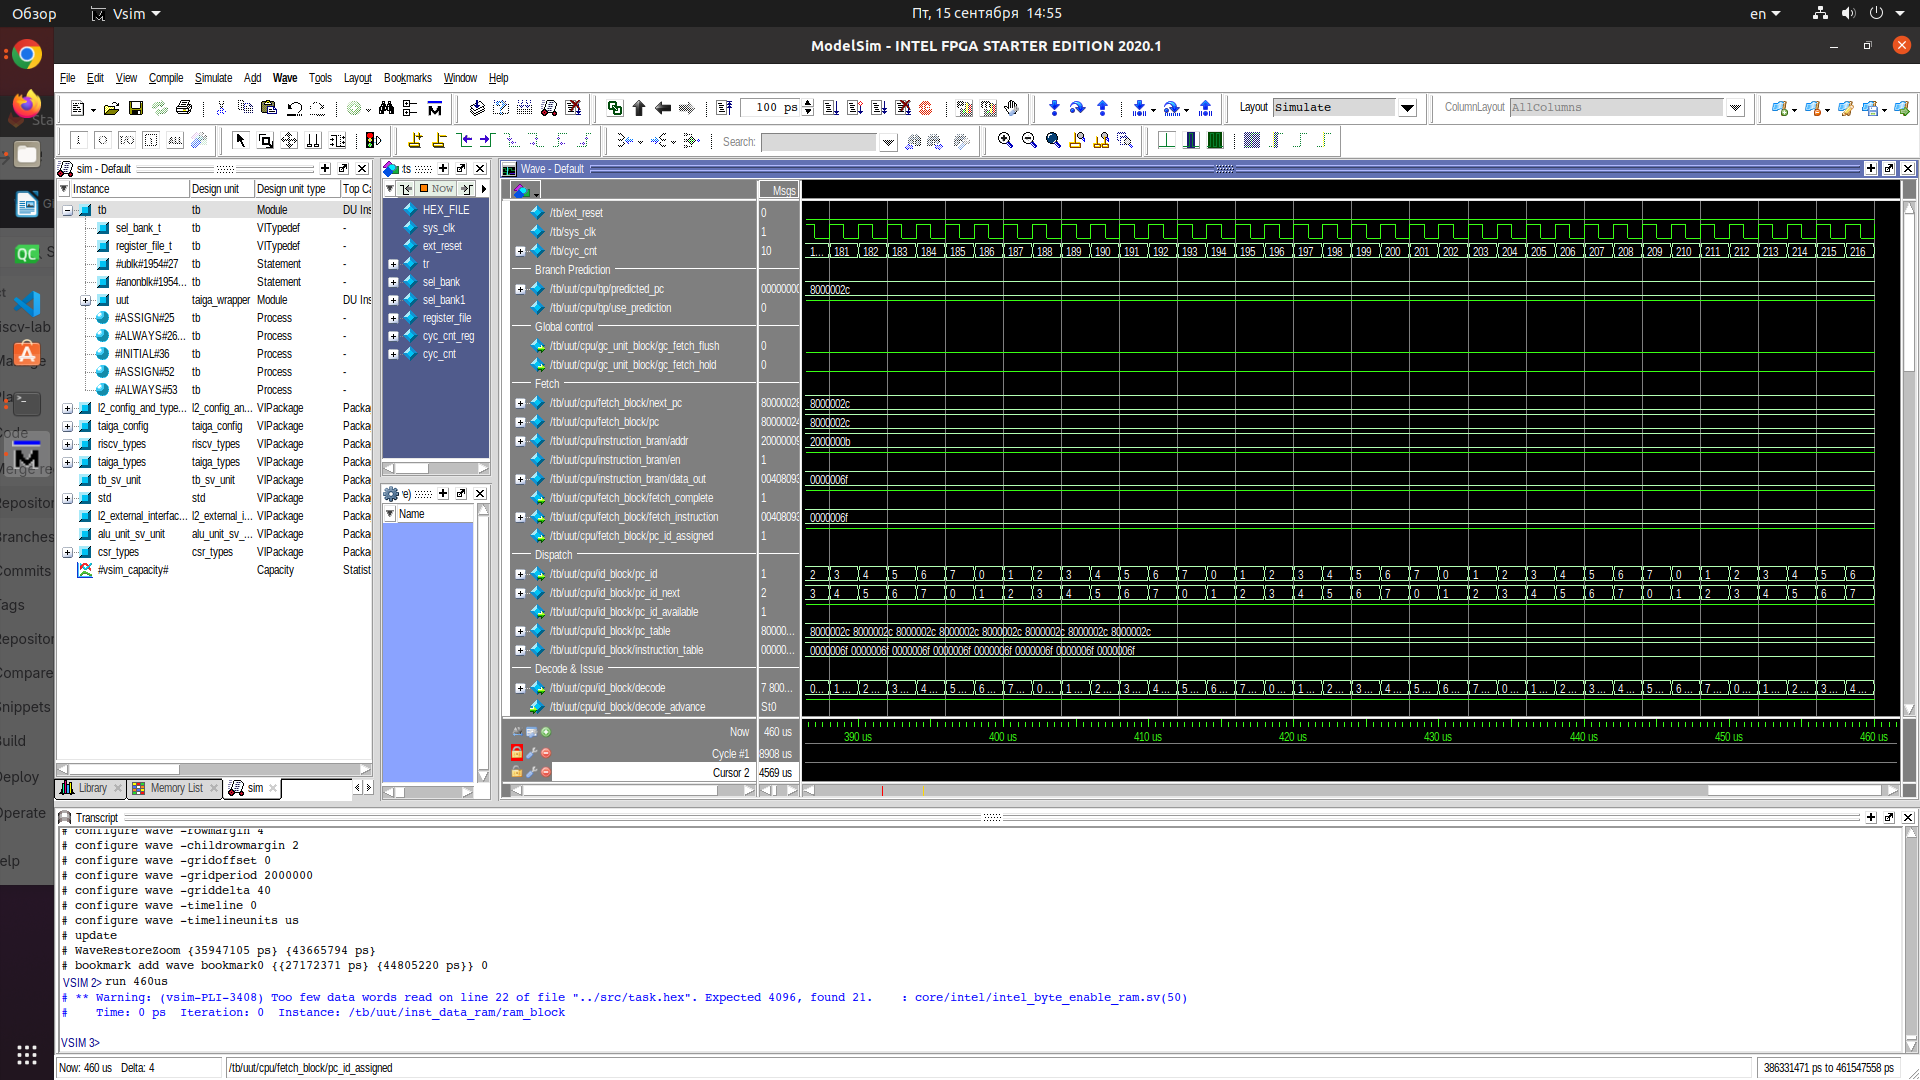
\includegraphics[width=170mm]{./img/task_5_1.png}
    \caption{Временная диаграмма \label{overflow5}}
\end{figure}

\begin{figure}[ht!]
    \centering
    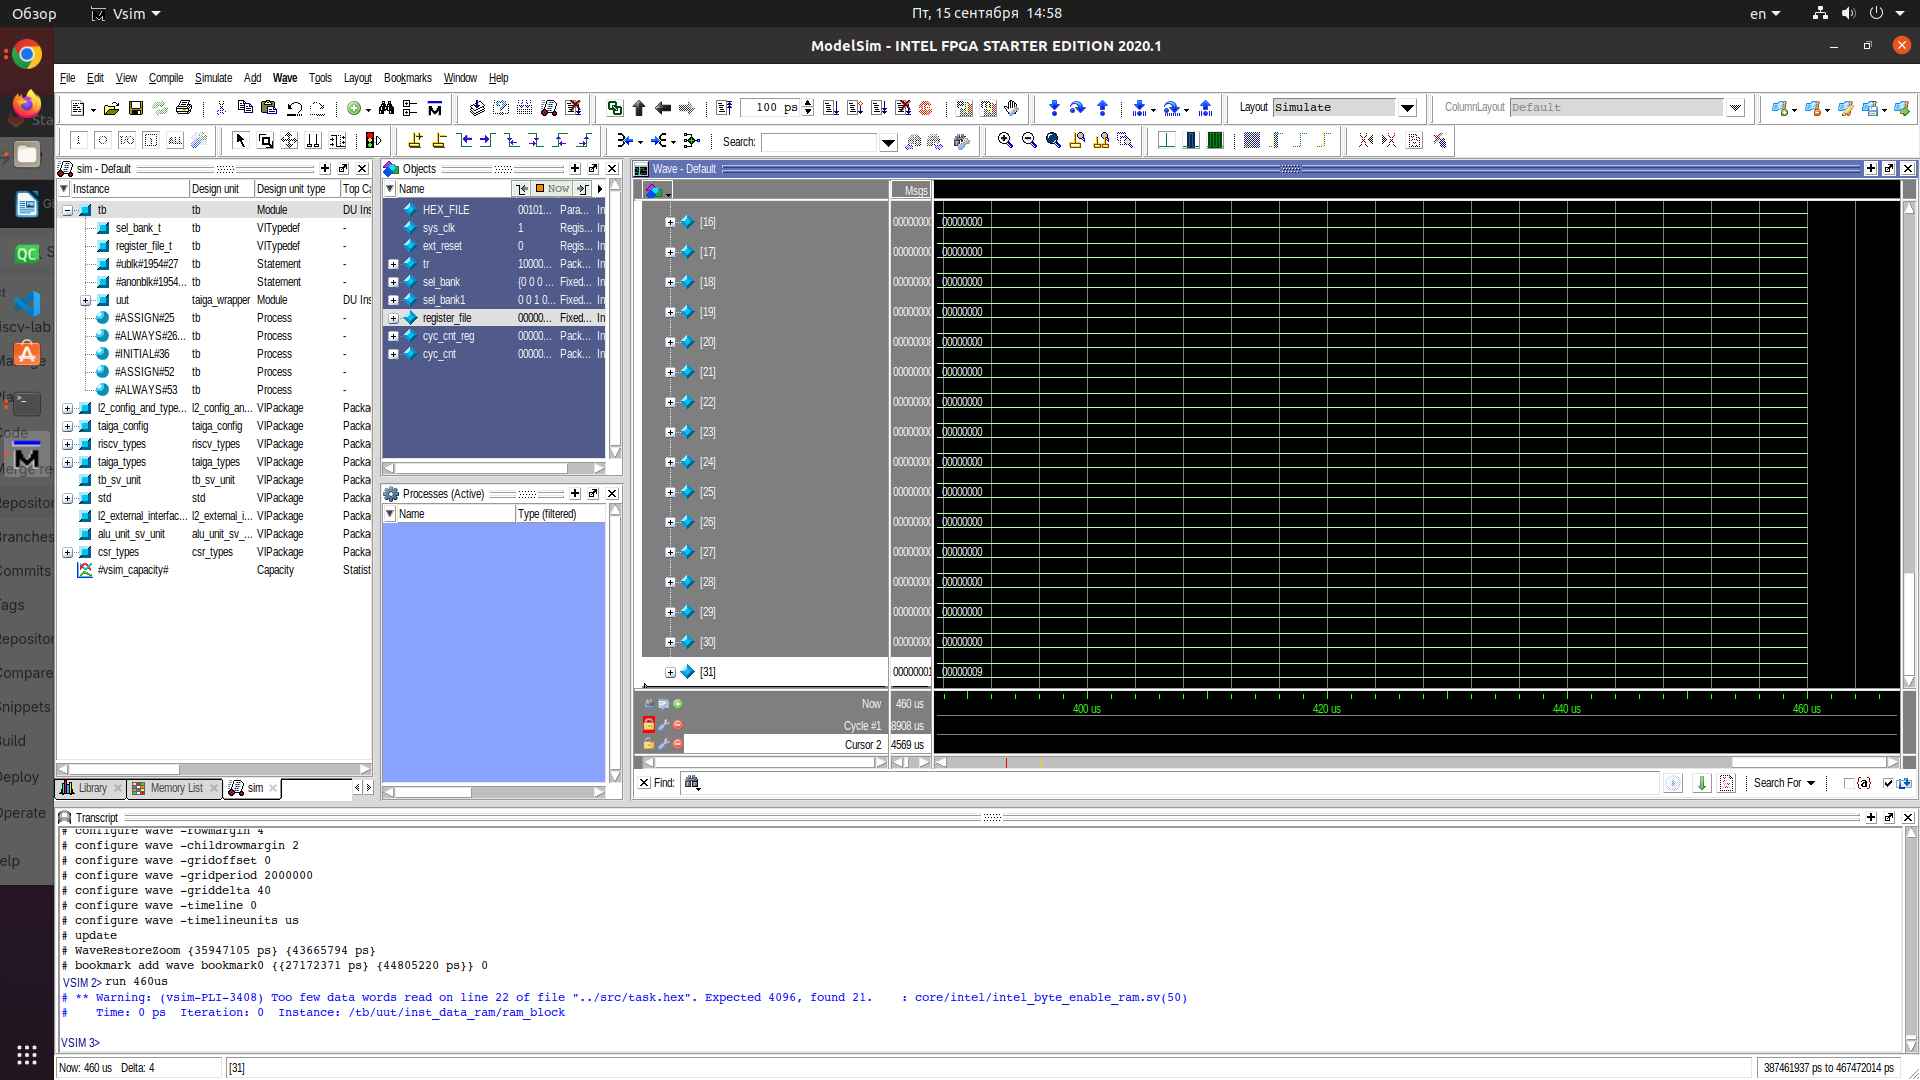
\includegraphics[width=170mm]{./img/task_5_2.png}
    \caption{Значение в register[31] \label{overflow6}}
\end{figure}

Заметим, что значение из регистра $x31$ совпадает с вычисленным ранее значением.

\begin{figure}[ht!]
        \centering
        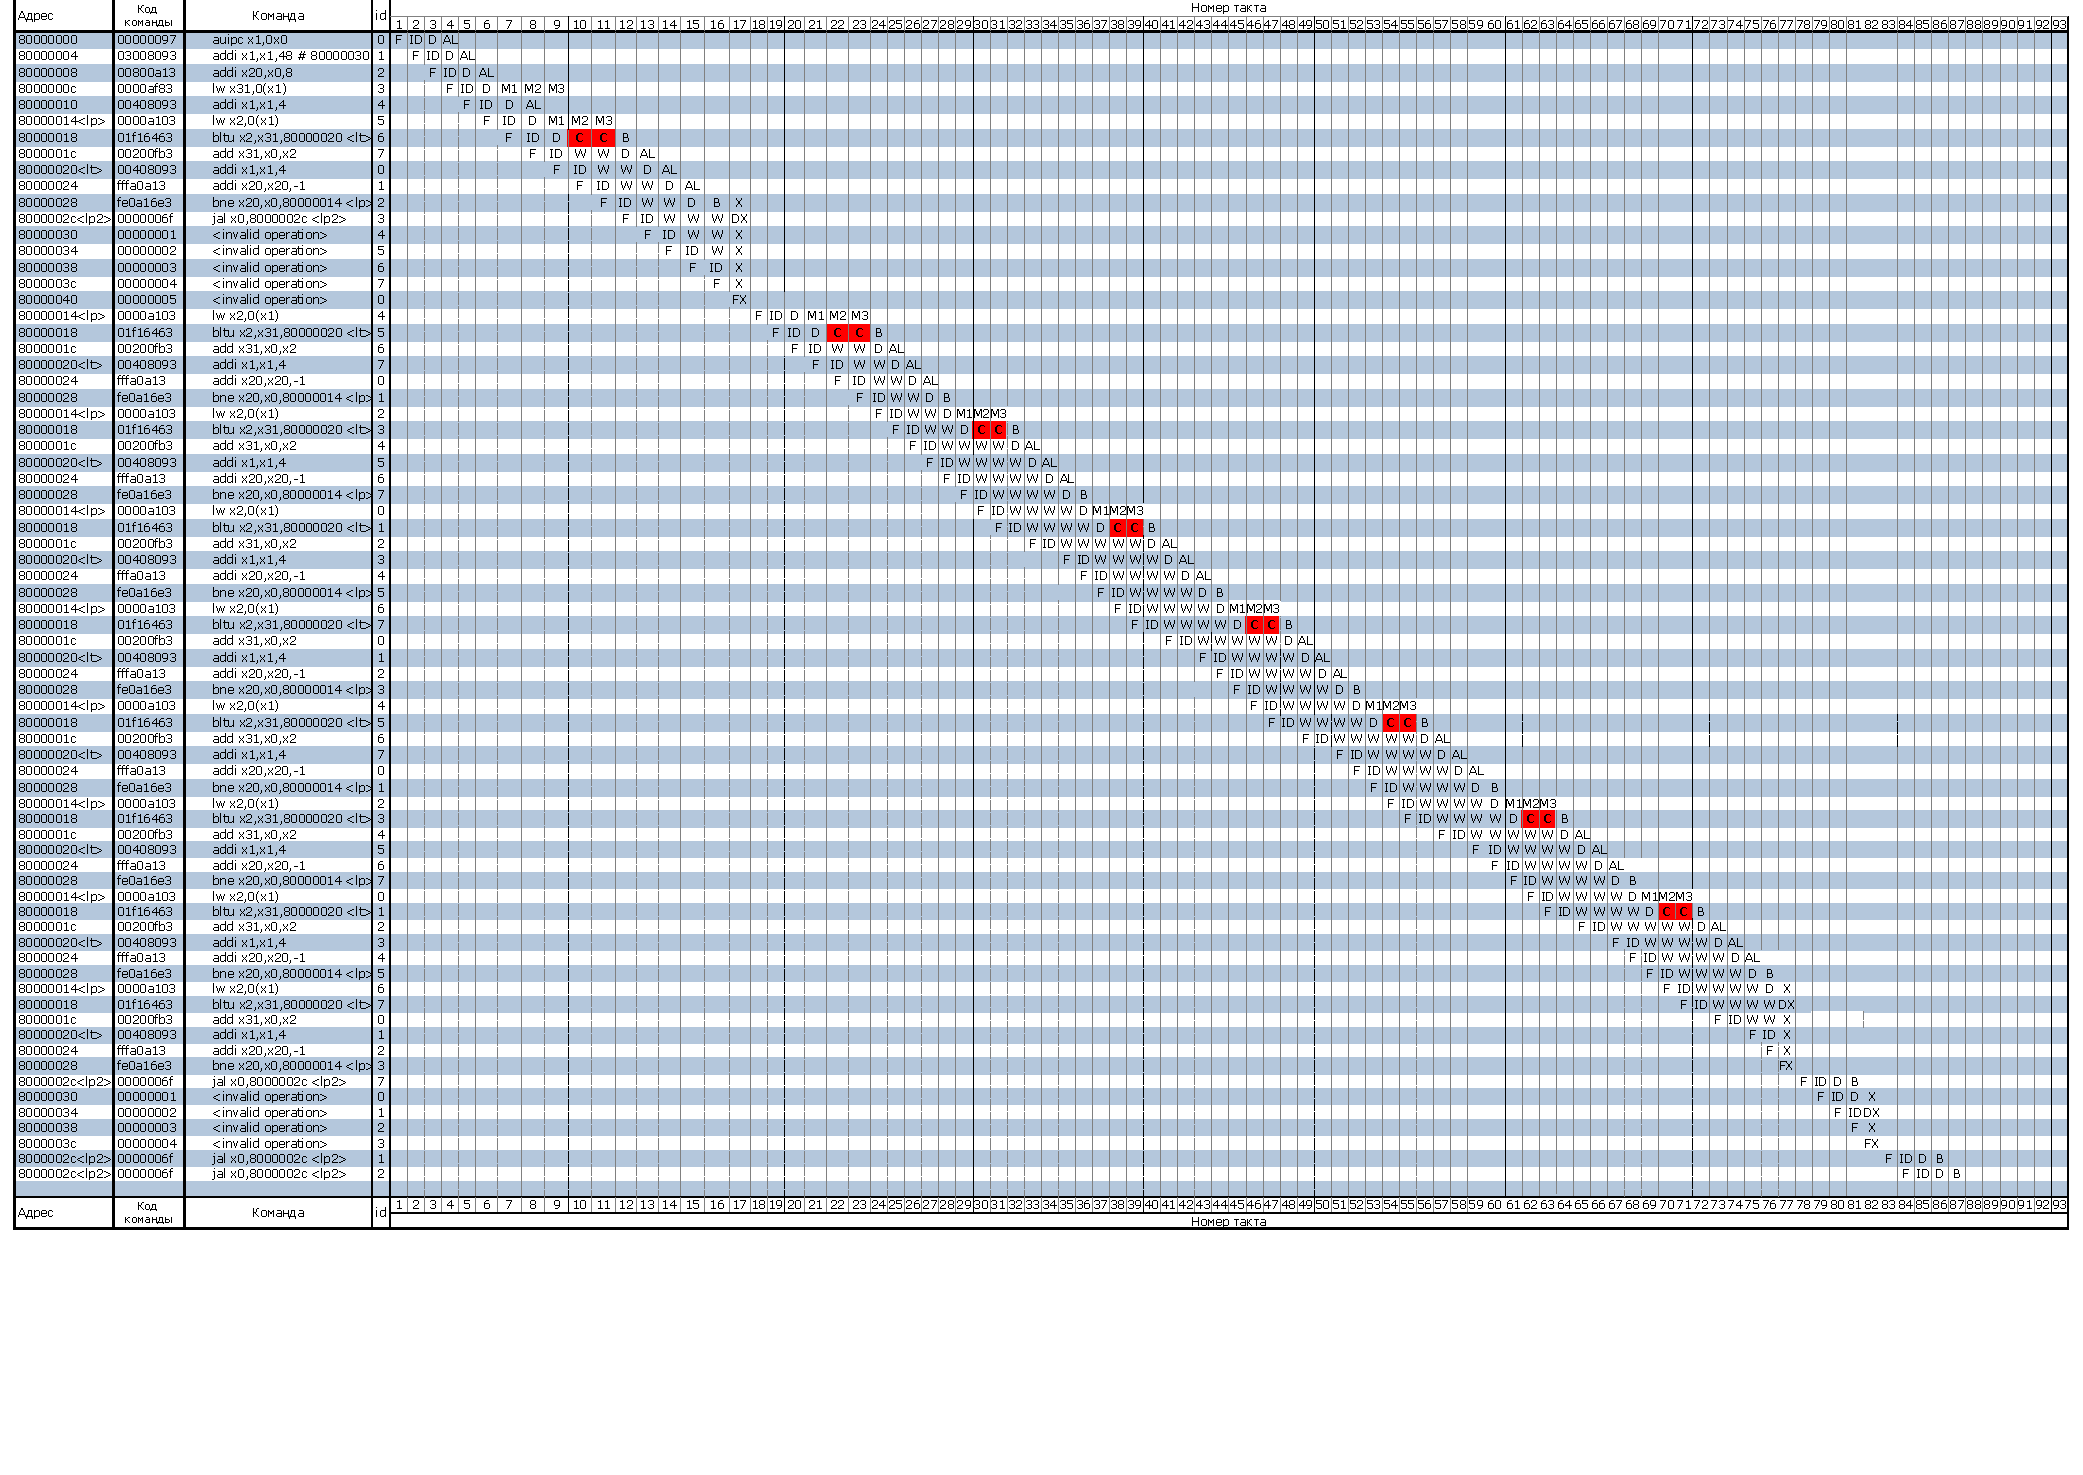
\includegraphics[width=170mm]{./trassa/default.pdf}
        \caption{Трасса работы программы\label{overflow7}}
    \end{figure}

Оптимизированная программа:
\begin{lstlisting}

.section .text
        .globl _start;
        len = 9 #Размер массива
        enroll = 1 #Количество обрабатываемых элементов за одну итерацию
        elem_sz = 4 #Размер одного элемента массива

_start:
        la x1, _x
        addi x20, x0, (len-1)/enroll
        lw x31, 0(x1)
        addi x1, x1, elem_sz*1
lp:
        lw x2, 0(x1)
        
        add x1, x1, elem_sz*enroll
        addi x20, x20, -1

        bltu x2, x31, lt
        add x31, x0, x2 #!
lt:
        bne x20, x0, lp
lp2: j lp2

        .section .data
_x:     .4byte 0x1
        .4byte 0x2
        .4byte 0x3
        .4byte 0x4
        .4byte 0x5
        .4byte 0x6
        .4byte 0x7
        .4byte 0x8
        .4byte 0x9

\end{lstlisting}

Трасса работы оптимизированной программы:
\begin{figure}[ht!]
    \centering
    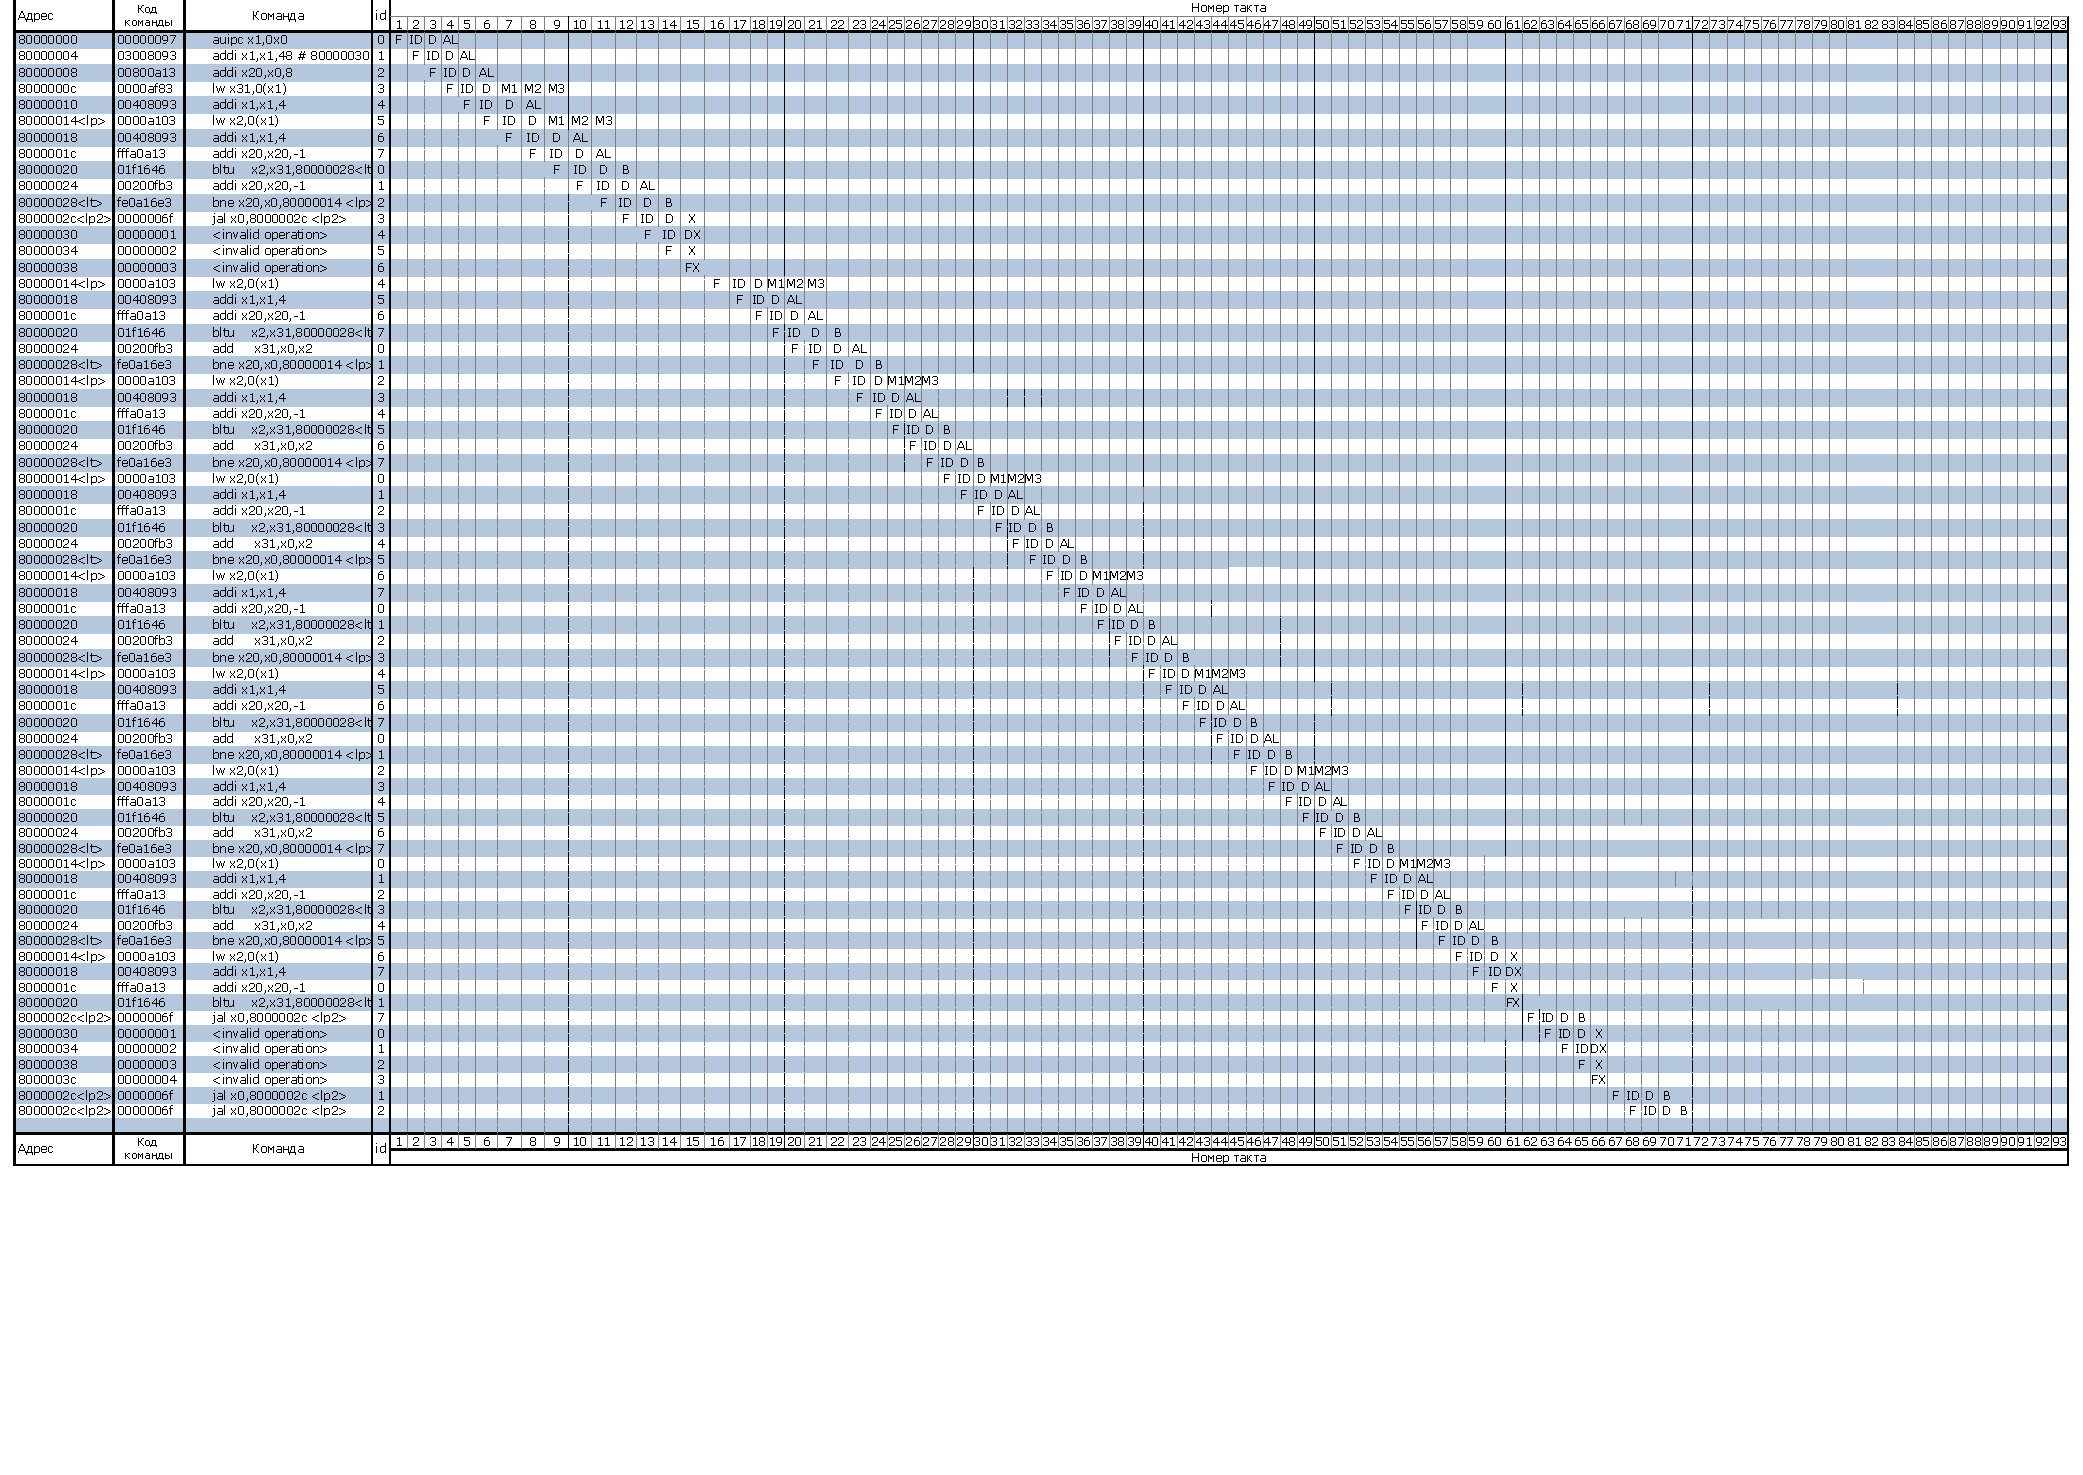
\includegraphics[width=170mm]{./trassa/opt.pdf}
    \caption{Трасса работы оптимизированной программы\label{overflow8}}
\end{figure}